\documentclass[11pt]{beamer}
\usepackage[OT1]{fontenc}
\usepackage[utf8x]{inputenc}
\usepackage[frenchb]{babel}
%\usepackage[dvipsnames]{xcolor}
\usepackage{xcolor}
\usetheme{PickEM}
\title{D\'eveloppement d'un utilitaire de s\'election de particules observ\'ees au microscope \'electronique}
\subtitle{Pick\_EM}
\date{Mai 2012}
\author{\textsc{Faux} - \textsc{Héricé} - \textsc{Paysan-Lafosse} - \textsc{Sansen}}
\institute[Universite Bordeaux 1 \& 2] 
 {
 Master 1 Bioinformatique \\ Projet de programmation sous la direction de Jean-Christophe \textsc{Taveau} \\ 
 \begin{figure}[h]
  \begin{center}
  
\includegraphics[width=0.25\columnwidth]{beamer/logounibdx.png}
  \hspace{1cm}
  
\includegraphics[width=0.3\columnwidth]{beamer/banniere_cbmn.png}
  \end{center}
 \end{figure}
 }
\begin{document}

\frame{\titlepage}
\section*{Sommaire}
\begin{frame}
  \tableofcontents
\end{frame}
\section{Introduction}
\begin{frame}
\frametitle{Introduction}
\begin{block}{CBMN}
Laboratoire de Chimie et Biologie des Membranes et Nanoobjets 
\end{block}
\begin{block}{ACMPC}
\'Equipe Architectures des Complexes Membranaires et Processus Cellulaires
\end{block}
\end{frame}

\subsection{Contexte}
	\begin{frame}
	\frametitle{Introduction - Contexte}
	\begin{itemize}
		\item Micrographies de structures protéiques issue de MET
		\item Utilisation du logiciel ImageJ
		\item Sélection manuelle fastidieuse 
		\begin{itemize}
			\item Chronophage
			\item Accapare un membre de l'equipe
			\item Répétitive
		\end{itemize}
	\end{itemize}
	\begin{figure}
		\includegraphics[scale=0.05]{beamer/base.jpg}
		
		Exemple de micrographie
	\end{figure}
\end{frame}

\subsection{Objectif}
\begin{frame}
\frametitle{Introduction - Objectif}
	\begin{columns}[t]
		
		\begin{column}{4.5cm}
			\begin{block}{Création d'une interface}
				\begin{itemize}
					\item Facile d'utilisation
					\item Claire et succinte
					\item Récupération des paramètres utilisateurs
				\end{itemize}
			\end{block}
		\end{column}
		\begin{column}{6.5cm}
		    \begin{block}{Implémentation d'algorithmes}
				\begin{itemize}
					\item Automatisation du traitement
					\item Récupération des coordonnées
					\item Images résultantes
				\end{itemize}
			\end{block}
		\end{column}
	\end{columns}
\end{frame}

\section{Analyse}
\subsection{Besoins Fonctionnels}
\begin{frame}
\frametitle{Analyse - Besoins Fonctionnels}
	\begin{columns}[t]
		
		\begin{column}{5cm}
			\begin{block}{Interface}
				\begin{itemize}
					\item Choix entre plusieurs algorithmes
					\item Diffère entre chaque algorithme
				\end{itemize}
			\end{block}
		\end{column}
		\begin{column}{5cm}
			\begin{block}{Algorithmes}
				\begin{itemize}
					\item Piquage automatique
					\item Résultats : tableau de coordonnées (x, y, z) et images résultantes
				\end{itemize}
			\end{block}
		\end{column}
	\end{columns}	
\end{frame}

\subsection{Besoins non Fonctionnels}
\begin{frame}
\frametitle{Analyse - Besoins non Fonctionnels}
	\begin{columns}[t]
		\begin{column}{5cm}
			\begin{block}{Algorithmes}
				\begin{itemize}
					\item Implémentation en Java (tests avec l'outil Macro d'ImageJ)
					\item Traitement rapide (grands jeux de données)
					\item Minimiser les étapes intermédiaires
				\end{itemize}
			\end{block}
		\end{column}
		\begin{column}{5cm}
			\begin{block}{Interface}
				\begin{itemize}
					\item Implémentation en Java (AWT ou \textbf{Swing})
					\item Modularité
				\end{itemize}
			\end{block}
		\end{column}
	\end{columns}
\end{frame}

\section{Conception - Réalisation}
\begin{frame}
\frametitle{Interface Graphique}
	\begin{columns}
		\begin{column}{6cm}
			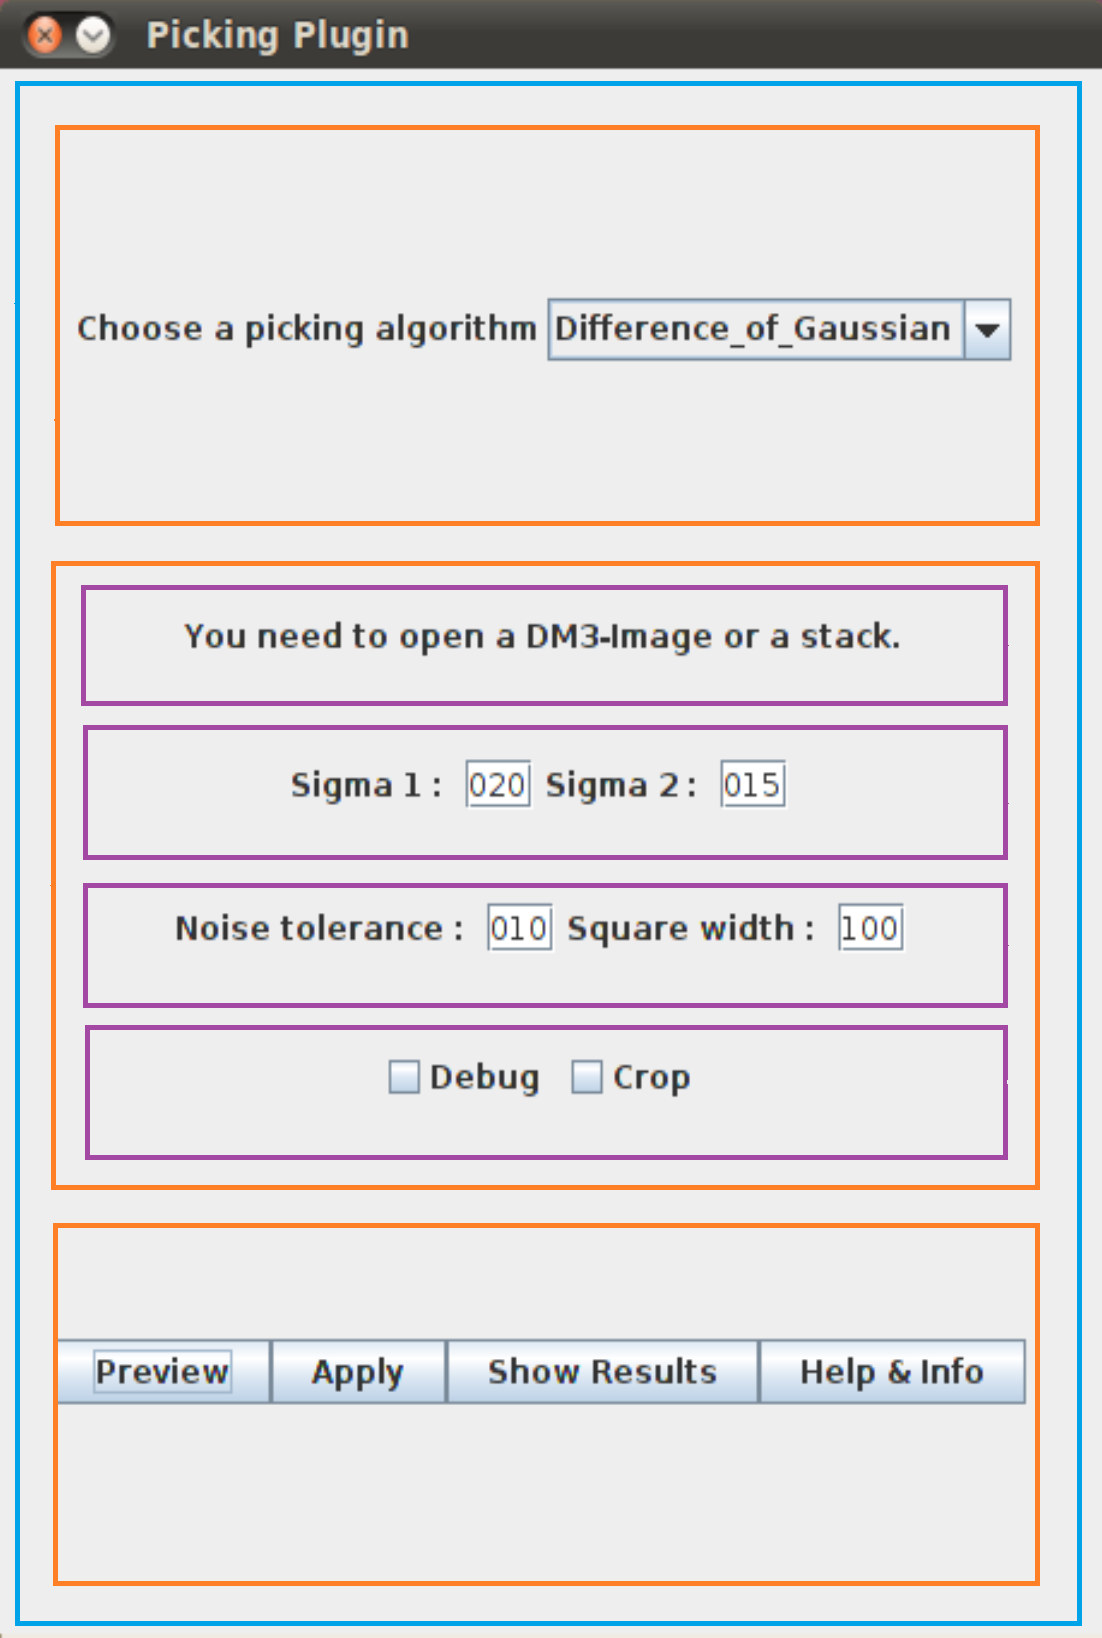
\includegraphics[scale=0.12]{beamer/pluginCadres.png}
		\end{column}
		\begin{column}{4cm}
			Organisation générale de l'interface
		\end{column}
	\end{columns}
\end{frame}
\begin{frame}
\frametitle{Récupération des paramètres utilisateurs}
	Patrons de Conception : \emph{Factory} et \emph{Singleton}
	\begin{columns}[t]
		\begin{column}{5cm}
			\begin{block}{Choix de l'algorithme}
				\begin{itemize}
					\item JComboBox
				\end{itemize}
			\end{block}
			\vspace*{2cm}
			\includegraphics[scale=0.45]{beamer/combobx.png}
		\end{column}
		\begin{column}{5cm}
			\begin{block}{Paramètres propres aux algorithmes}
				\begin{itemize}
					\item JTextField
					\item JCheckBox
				\end{itemize}
			\end{block}
			\includegraphics[scale=0.15]{beamer/param.png}
		\end{column}
	\end{columns}
\end{frame}
\begin{frame}
\frametitle{Démonstration avec la Différence de Gaussiennes (DoG)$~$ Wouf!}
	\begin{columns}
		\begin{column}{5cm}
			\begin{figure}
				\includegraphics[scale=0.07]{beamer/base.jpg}
	
				Micrographie de protéines transmembranaires
			\end{figure}
		\end{column}
		\begin{column}{5cm}
			\begin{itemize}
				\item Application de filtres gaussiens
				\item Soustraction des images filtrées
				\item Récupération des maxima
				\item Extrapolation des points sélectionnés sur l'image de bases
			\end{itemize}
		\end{column}
	\end{columns}
\end{frame}
\begin{frame}
\frametitle{Algorithmes}
	\begin{columns}
		\begin{column}{5cm}
			\begin{figure}
				\includegraphics[scale=0.07]{beamer/filtreGaussien15.jpg}
				
				Filtre Gaussien (Radius 15)
			\end{figure}			
		\end{column}
		\begin{column}{5cm}
			\begin{figure}
				\includegraphics[scale=0.07]{beamer/filtreGaussien20.jpg}
				
				Filtre Gaussien (Radius 20)
			\end{figure}
		\end{column}
	\end{columns}
\end{frame}
\begin{frame}
\frametitle{}
\begin{columns}
\begin{column}{5cm}
			\begin{figure}
				\includegraphics[scale=0.07]{beamer/resultsubstractgaussian.jpg}
				
				Résultat de la soustraction
			\end{figure}
\end{column}
\begin{column}{5cm}
			\begin{figure}
				\includegraphics[scale=0.14]{beamer/gaussianmaxima.jpg}
				
				Résultat du maxima
			\end{figure}
\end{column}
\end{columns}
\end{frame}
\begin{frame}
\frametitle{Résultats}
	\begin{columns}
		\begin{column}{5cm}
			\begin{figure}
				\includegraphics[scale=0.13]{beamer/imgCrop.png}
				
				Résultat du piquage
			\end{figure}
		\end{column}
		\begin{column}{5cm}
			\begin{figure}
				\includegraphics[scale=0.12]{beamer/cropall.png}
				
				Images individuelles et tableaux de coordonnées
			\end{figure}
		\end{column}
	\end{columns}
\end{frame}
\section{Conclusion}
\begin{frame}
\frametitle{Conclusion}
\end{frame}

\begin{frame}
\frametitle{Remerciements}
\begin{block}{Merci!!! ;-)}
merci beaucoup pour votre attention!
\end{block}
\end{frame}

\end{document}